%!TEX TS-program = pdflatex
%!TEX root = i3det-top.tex
%!TEX encoding = UTF-8 Unicode

% additional definitions
\newcommand{\degC}[1]{$\unit[#1]{^\circ{C}}$}
% definition to produce a "less than or similar to" symbol
\def\lsim{\mathrel{\rlap{\raise 0.2ex\hbox{$\,<\,$}}{\lower 0.9ex\hbox{$\,\sim\,$}}}}
% definition to produce a "greater than or similar to" symbol
\def\gsim{\mathrel{\rlap{\raise 0.2ex\hbox{$\,>\,$}}{\lower 0.9ex\hbox{$\,\sim\,$}}}}


\section{\label{sec:dom}The Digital Optical Module}

\subsection{\label{sec:dom_functional}A Functional Description of the DOM}

The DOM is the fundamental light sensor and data acquisition unit for IceCube.
It consists of a spherical glass housing 
containing a downward-facing \SI{10}{''} diameter PMTs~\cite{ICECUBE:PMT}
and associated circuit boards that allow near-autonomous operation (Figure~\ref{fig:domcomponents}).
Data acquisition, control, calibration, communication, and low voltage power conversion 
are integrated in one annular circuit board (Main Board) that fits around the neck of the PMT~\cite{ICECUBE:DAQ}. 
Separate circuit boards generate PMT high voltage, interface to the PMT pin,
delay PMT signals, and generate calibration light flashes that can reach other DOMs.
Key requirements for the DOM include
the precise recording of a wide variety of PMT pulse widths and amplitudes with nanosecond time resolution, robustness in
a challenging deployment environment, and long-term reliability.

%============================================================

\begin{figure}[!h]
  \captionsetup[subfigure]{labelformat=empty}
  \centering
  \subfloat[]{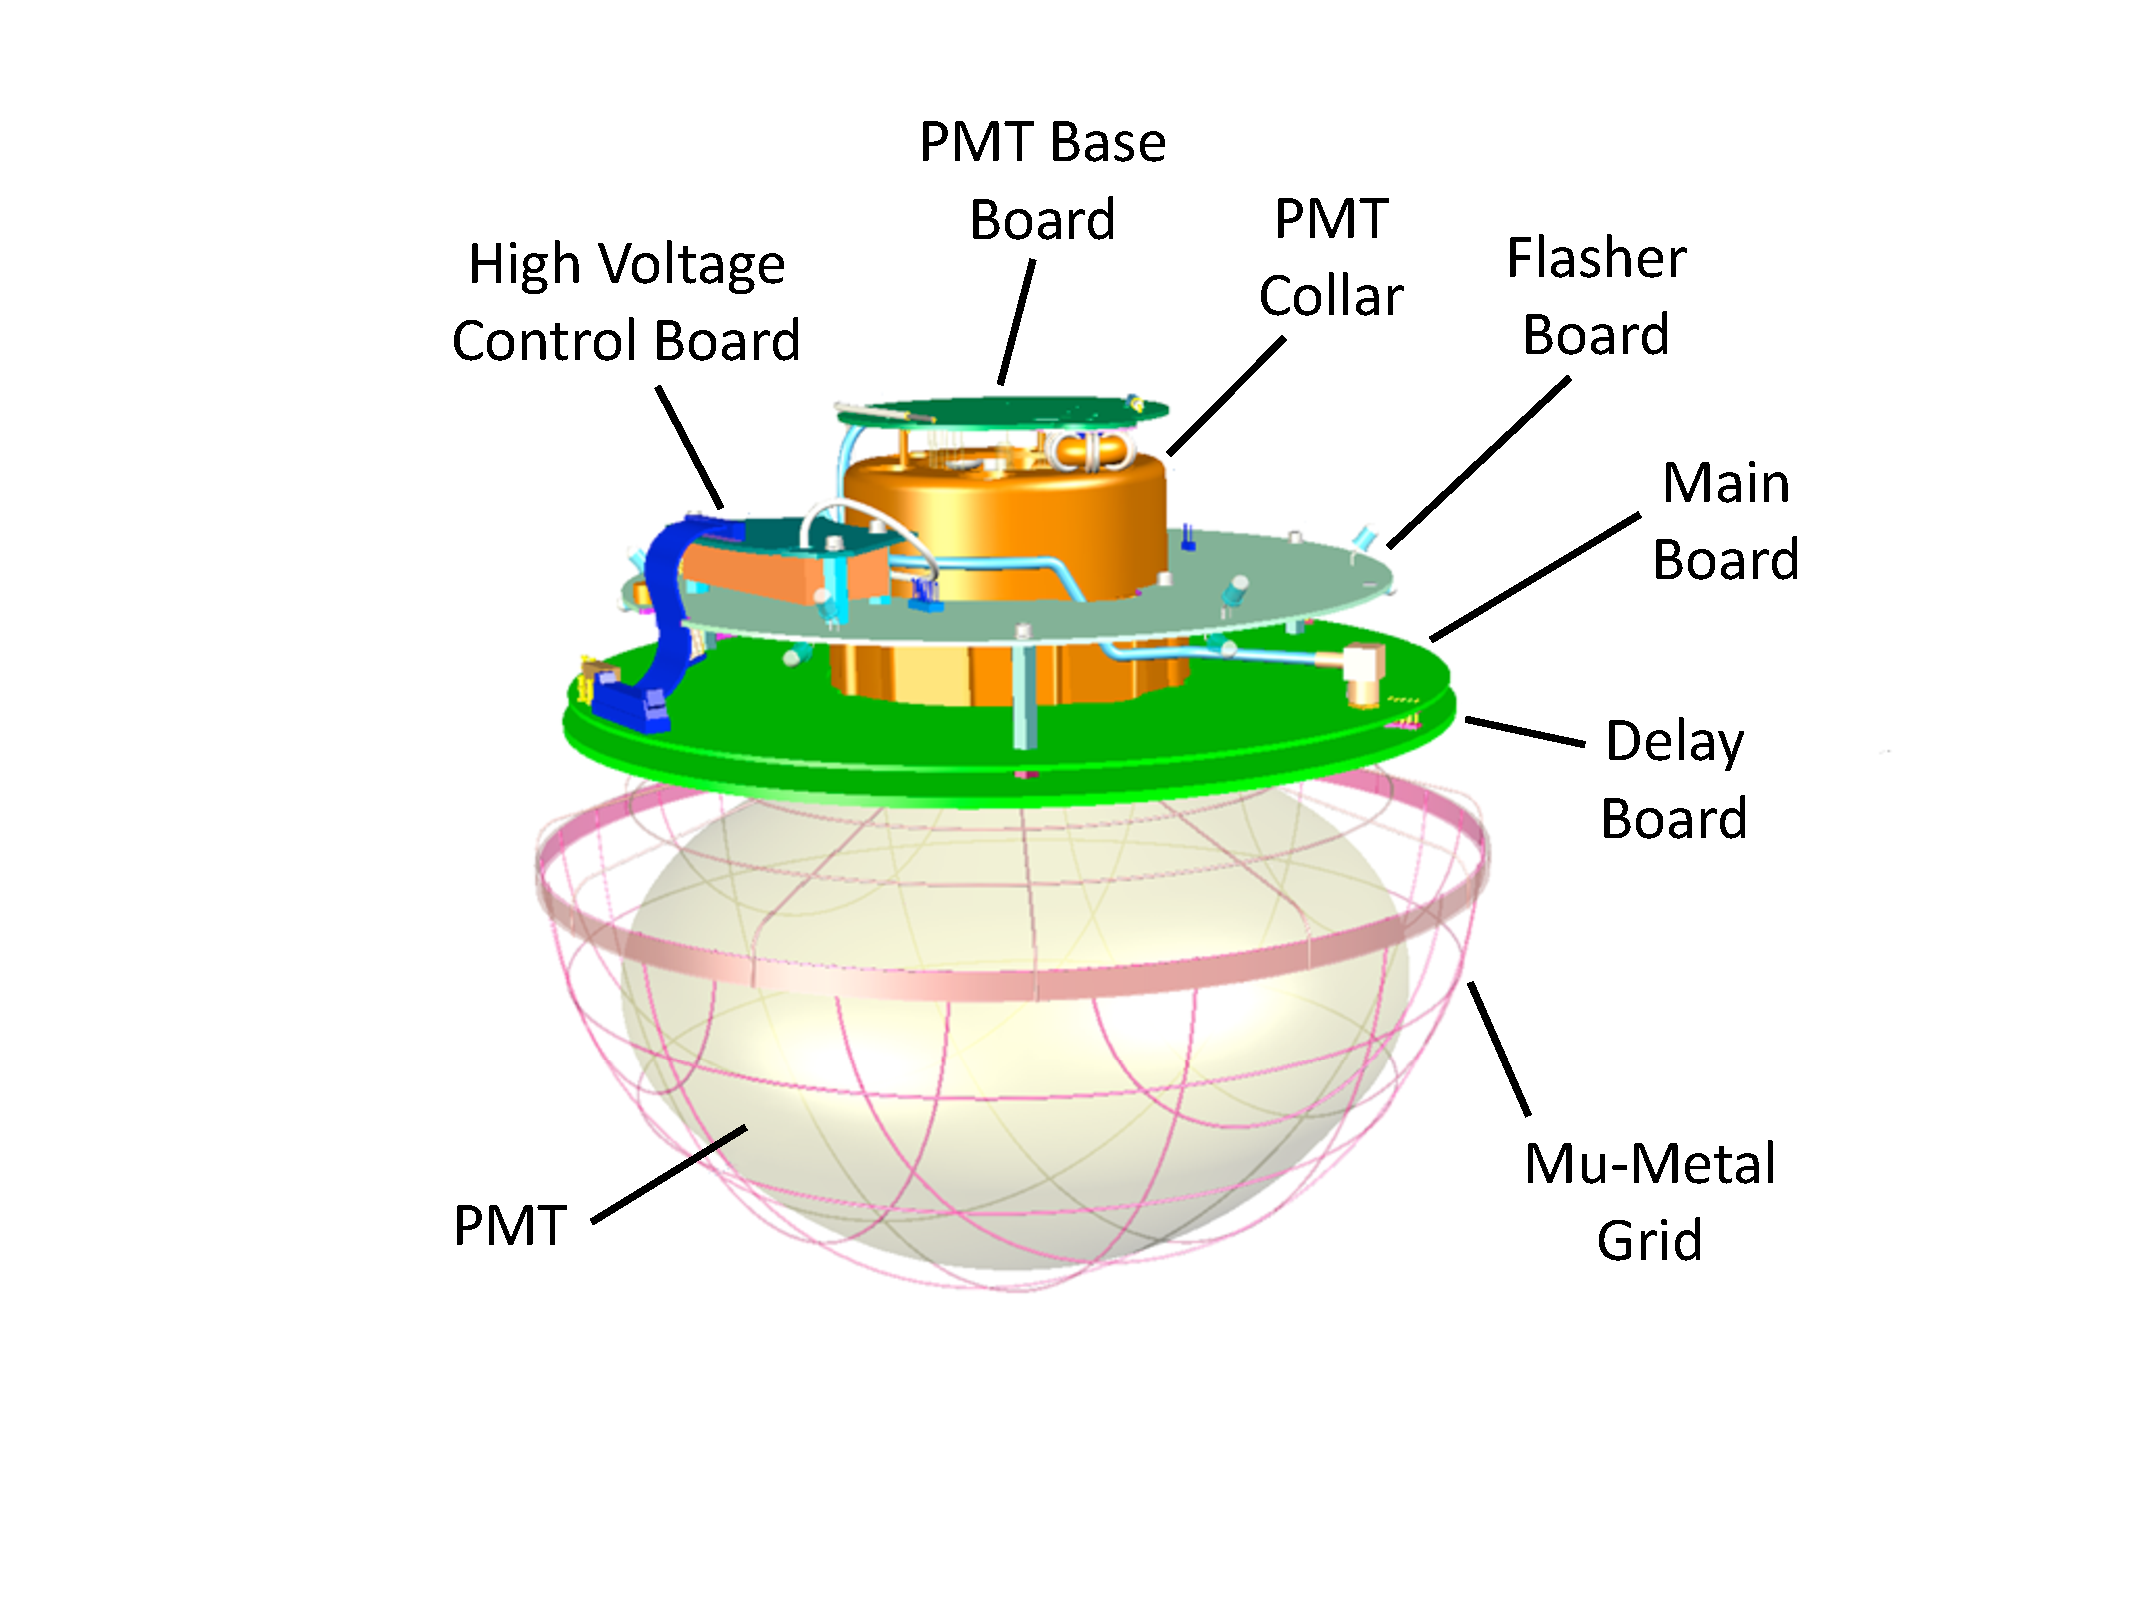
\includegraphics[width=0.5\textwidth]{graphics/dom/functional/domfig1a-DOM3DModel.pdf}}
  \subfloat[]{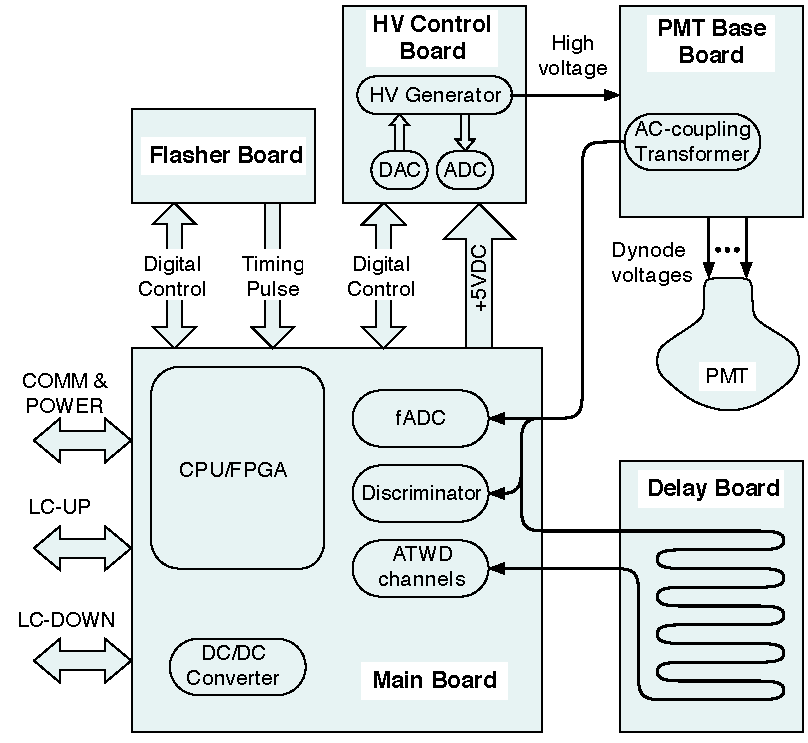
\includegraphics[width=0.5\textwidth]{graphics/dom/functional/domfig1b-DOMBlockDiagram.pdf}}
  \caption{Components of the DOM, showing mechanical layout (left) and functional connections (right).}
  \label{fig:domcomponents}
\end{figure}

%============================================================


The PMT detects signals from particles interacting the ice, typically ranging over
energies from \unit[10]GeV to \unit[10]PeV and distances up to \unit[500]m
away.  At a gain of $10^7$ (see Sec.~\ref{sec:hv}), corresponding PMT waveforms can have amplitudes from \unit[1]mV up
to and beyond the linearity limit of the PMT (\unit[$\sim2$]V) and widths
from \unit[12]ns to \unit[1500]ns.  In order to accommodate such a variety
of signals, the DOM includes multiple digitizers with overlapping dynamic
range and different sampling speeds
(Sec.~\ref{sec:mainboard}).  Each DOM independently
detects individual photons, starting a recording of
the PMT waveform that also includes photons arriving up to
\unit[6.4]{$\mu$s} later (a ``hit'').  The hit time is saved along with the
waveform shape, allowing the determination of the times of arriving photons
relative to this reference.  The DOM accumulates such hit
data for a period of \unit[1]s before sending the data up as a block.
However, if data readout is interrupted, the DOM can store
$\mathcal{O}(\SI{10}{\second})$ of data before overflowing local memory
(16MB of SDRAM), depending on hit rate.  Separately, the PMT hit rate is recorded by
the DOM in \unit[1.6384]ms intervals, as a collective increase of all rates
could signify detection of many low energy neutrinos in case of a Galactic
supernova event (see Sec.~\ref{sect:SNDAQ}).

DOMs transmit their data to computers in the IceCube Laboratory building (ICL)
using a twisted wire pair that also provides power (Sec.~\ref{sec:cable}).
Wire pairs are bundled to form the vertical in-ice cables and the horizontal surface
cables.  Each wire pair is shared between two DOMs, with data transfers
initiated by a surface computer.  Separately, dedicated local coincidence
(LC) wiring to neighbor DOMs above and below allows quick recognition of neighboring
coincident hits, where
nearest or next-to-nearest neighbors are hit within a common time
window. The time window is configurable and is set to  \unit[1]$\mu$s
for both in-ice and IceTop DOMs. The signals are forwarded from one DOM to the next
through the dedicated wiring; the span of the forwarding is
software-configurable and is currently set to two for in-ice DOMs,
i.e. a DOM signals its neighbor and next-to-nearest neighbor DOMs in
both up and down directions along the string. The local coincidence
connections for IceTop, which allow coincidences between the two tanks in a
station, are described in Ref.~\cite{ICECUBE:IceTop}. Local coincidence
hits (``HLC'' hits) often have complex PMT waveforms
indicating multiple photons detected in each DOM, which are therefore saved
in full detail; otherwise, the DOM saves abbreviated information appropriate
to single photon detection (see Sec.~\ref{sect:online:dataflow}).

The DOM is capable of interpreting commands from the surface that specify
tasks for configuration, data taking and transmission, monitoring or
self-calibration.  Self-calibration functions establish PMT and amplifier
gains as well as sampling speed (Sec.~\ref{sec:domcal}).  The RAPCal
system (Sec.~\ref{sect:dom:rapcal}) is implemented for tracking each
local DOM clock's offset from universal time, allowing PMT pulses that were
independently recorded in many DOMs to be built into events by surface
computers.

\subsection{\label{sec:dom_components}Components}

\subsubsection{\label{sec:sphere}Glass Sphere and Harness}

The glass sphere housing has an outer diameter \SI{13}{''} and thickness \SI{0.5}{''}.
The spheres are specified to protect the inside electronics and PMT against long-term applied pressure of 
\unit[250]bar (\unit[2.6]km equivalent water depth)
as well as temporary overpressure up to \unit[690]bar during the refreezing of melted ice in the drill hole.
The housings were produced by Benthos, Inc., based on a design for deep-sea
environments but using borosilicate glass from Kopp Glass
with very low potassium or other radioactive trace elements that would contribute to the dark noise
count rate (Sec.~\ref{sect:darknoise}).  
Optical transmission was measured in representative glass samples as 93\% at \unit[400]nm,
decreasing to 50\% at \unit[340]nm and 10\% at \unit[315]nm (normal
incidence). Fresnel reflection is not included in the quoted
transmission, since the effect of Fresnel reflection is small in ice,
where the refractive index is better matched to the glass.

%N.B. not borosilicate, according to analysis shown at final CDR 2005 (Claire's slides), in contrast
%to the Benthos sphere datasheet which says borosilicate.
% ACTUALLY is borosilicate, analysis can't detector boron

All spheres were tested up to \unit[690]bar hydrostatic pressure by the manufacturer.
Each was delivered as two hemispheres that mate precisely at the equator
and were sealed during assembly (Sec.~\ref{sec:dom_prodtest}).  The DOM
is held by an aluminum waistband with rubber gaskets against 
the glass above and below the equator seam. 
Fig.~\ref{fig:domcable} shows how the DOM is attached to the main in-ice cable via a harness
of steel rope and chain that carries the weight load around the DOM.
The main cable bends around the DOM, and the DOM axis stays vertically aligned with the string.

%============================================================
\begin{figure}
\vspace{3pt}
\centering
\begin{tabular}{c@{\hspace{0.5in}}c}
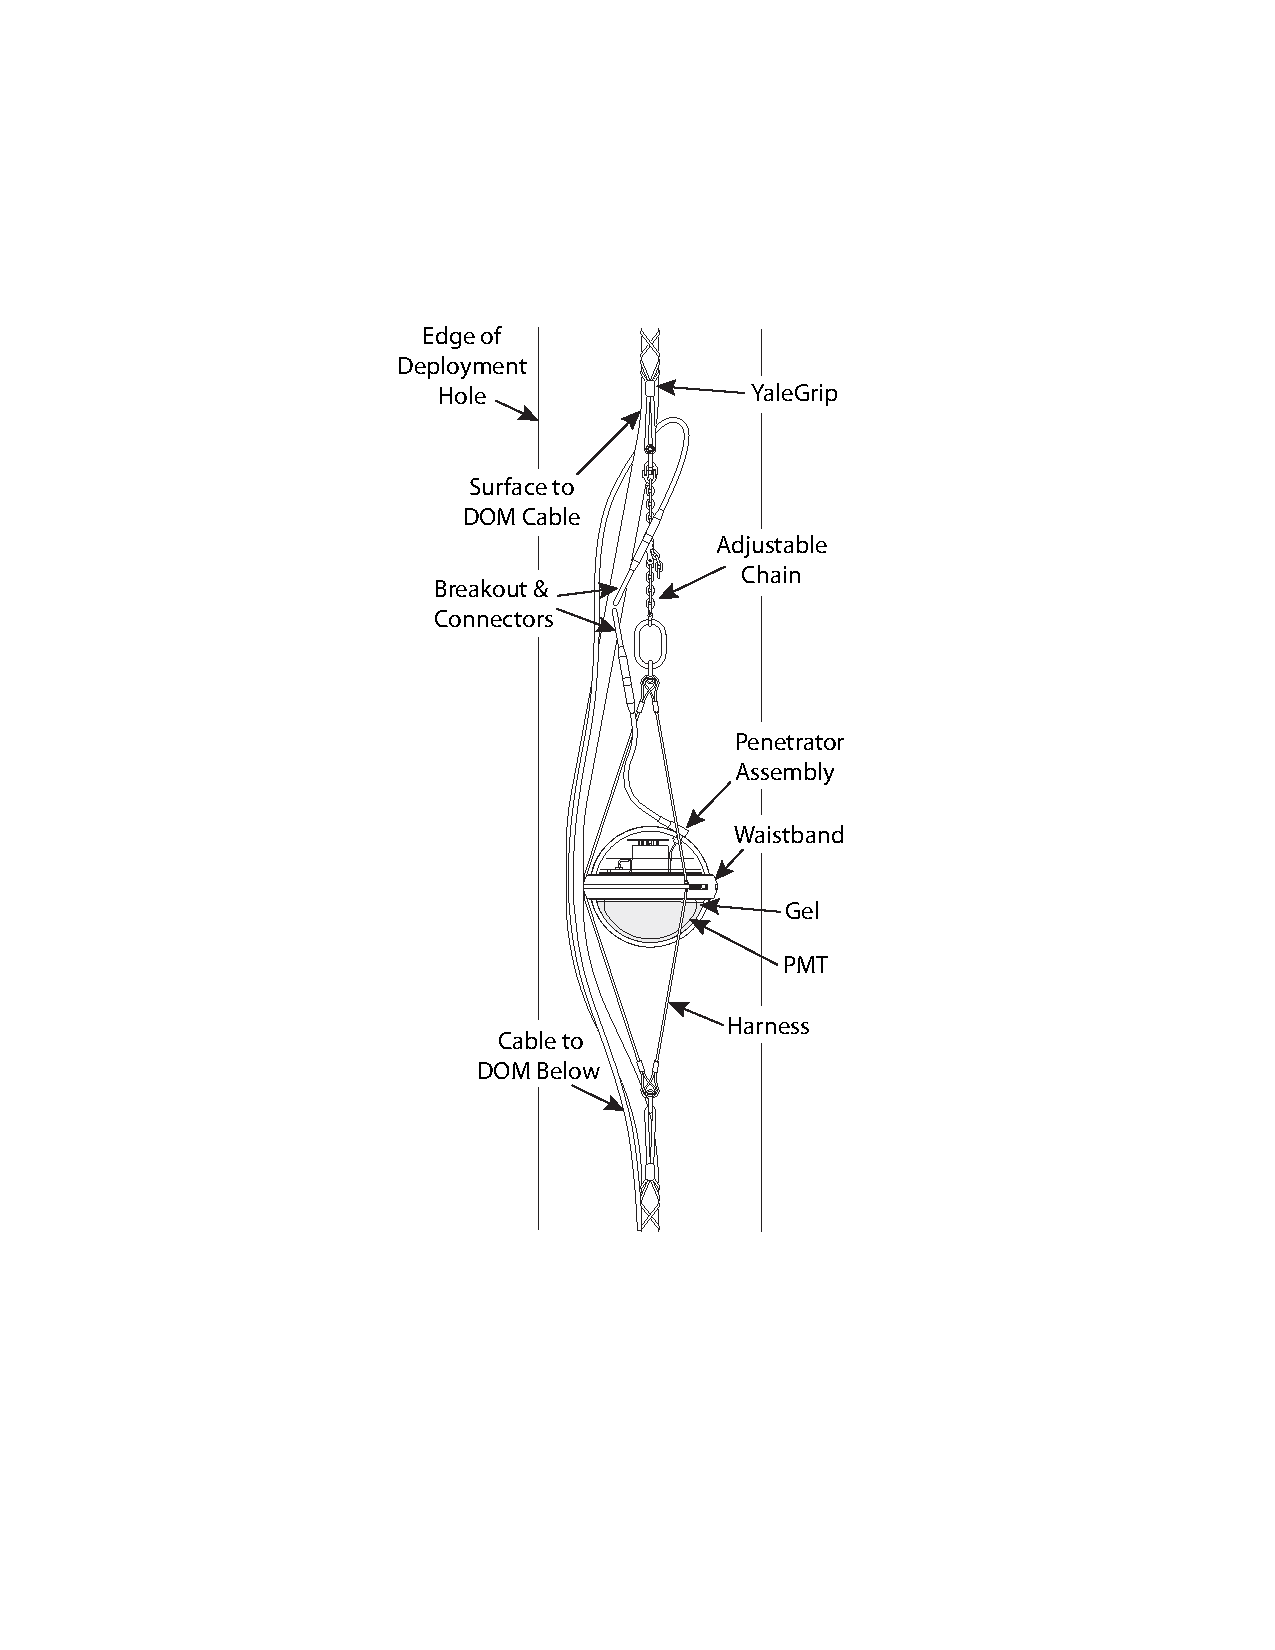
\includegraphics[width=0.4\textwidth,clip=true]{graphics/dom/functional/domfig2a-CableAssembly.pdf} & \
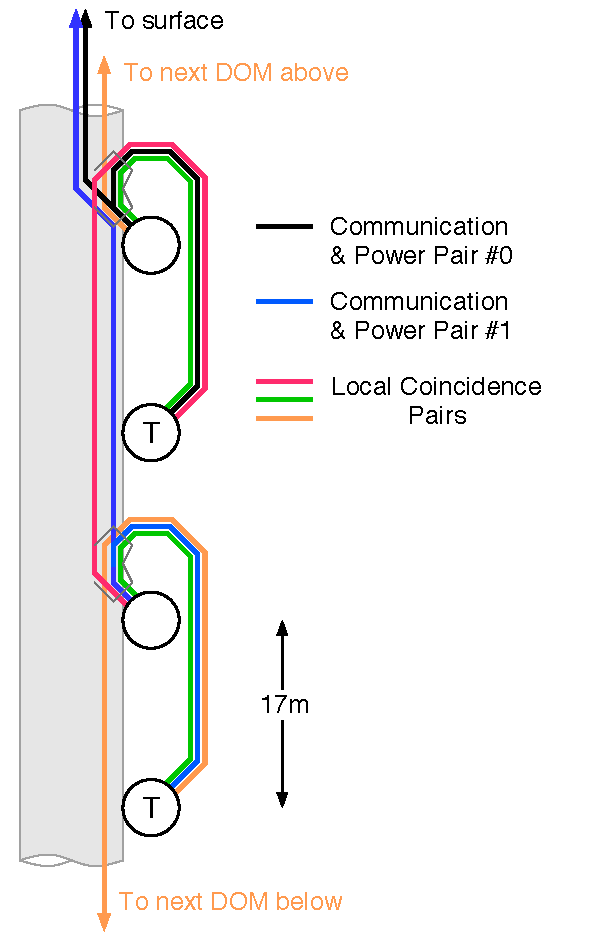
\includegraphics[width=0.45\textwidth,clip=true]{graphics/dom/functional/domfig2b-CableConnections.pdf} \\
\end{tabular}
\caption{
(Left) DOM as deployed on main in-ice cable, showing cable breakout to the penetrator
assembly and the mechanical support system.  (Right) Schematic of cable connections for a set
of four DOMs serviced by two wire pairs from the surface that carry power and
communications.  The ``T'' labels indicate where electrical termination (\unit[140]$\Omega$) is
installed in one of two DOMs that share such a wire pair.  Other wire pairs are used for
bidirectional signaling between neighboring DOMs, in order to check for in-time coincident
detections.
}
\label{fig:domcable}
\end{figure}
%============================================================

\subsubsection{\label{sec:penetrator}Cable Penetrator, Cable and Connector}

A penetrator assembly brings three wire pairs out through a \unit[16.3]mm hole in
the DOM glass.  They are routed inside a customized cable, shown in Fig.~\ref{fig:domcable},
and terminate at a pressure-tight, waterproof connector that mates with a similar connector
that continues each pair into the main cable.  One wire pair carries power and a
bidirectional digital communications stream, connecting ultimately
with a computer in the
IceCube Laboratory building (Sec.~\ref{sec:cable}).
The other wires lead to neighboring DOMs directly above and below,
carrying LC digital pulses that signify time-correlated hits in nearby DOMs (Sec.~\ref{sec:mainboard}).

DOMs were produced in two versions, in which the communications wire pair was either electrically
terminated (\unit[140]$\Omega$) or unterminated inside the DOM.  The
terminated DOM is deployed \unit[17]m below the unterminated one (\unit[7]m
or \unit[10]m in DeepCore strings) and therefore includes a correspondingly 
long penetrator assembly cable (Figure~\ref{fig:domcable}).

The entire penetrator assembly was designed and produced by SEACON
(California).  The part that seals against the DOM glass is a
hollow steel bolt that is secured inside the DOM by a nut and spring
washer and compresses a fluorosilicone O-ring against the outside surface.
The steel part includes additional sealing around the wires that pass
through it.  Outside the DOM, a plastic shell is molded around the steel
and onto the cable jacket.  External mechanical features like the
penetrator are subject to large stresses during deployment and the
refreezing process; a right angle bend outside the DOM was included for
robustness, based on previous experience deploying AMANDA modules.

\subsubsection{\label{sec:pmt}PMT, Gel and Magnetic Shield}

DOMs use the \SI{10}{''}-diameter Hamamatsu R7081-02 PMT, 
or the corresponding high-quantum-efficiency (HQE) version, Hamamatsu R7081MOD, for DeepCore strings.
The PMT properties have been measured and described in Ref.~\cite{ICECUBE:PMT}.
The PMT is specified by Hamamatsu for the wavelength range
\unit[300]nm--\unit[650]nm, with peak quantum efficiency around 25\% (34\%
for HQE) near \unit[390]nm.  It features a box-and-line dynode chain with 10 stages,
with in-ice DOMs (both standard and HQE) operated at a gain of $10^7$ (Sec.~\ref{sec:domcal}).

The PMT bulb faces downwards in the bottom glass hemisphere, secured in high-strength 
silicone gel to a depth sufficient to surround the photocathode area.  
The gel provides both mechanical support for the whole assembly of PMT and circuit boards,
as well as good optical coupling.  
The gel thickness between PMT envelope and glass sphere is approximately \unit[1]cm.  
Originally the gel was supplied from General Electric as RTV6136-D1,
and later as a similar formulation from Quantum Silicones (Virginia, USA).  
It is optically clear with transmission 97\% at \unit[400]nm, 91\% at \unit[340]nm, and 65\% at \unit[300]nm
(normal incidence).  The refractive index is 1.41, yielding less than 0.1\% reflection as light
passes from the sphere glass into the gel and then into the PMT envelope.
The characteristics of the cured gel are specified to remain stable in the
temperature range $-70^\circ$C to $45^\circ$C.  Visual inspection of
non-deployed DOMs reveals no indication of crazing after more than 10
years, and studies of the long-term optical efficiency of deployed DOMs
reveal no measurable aging effects (Sec.~\ref{sec:optical_stability}).  

To reduce effects of the ambient South Pole magnetic field (\unit[550]mG, $17^\circ$
from vertical) on the PMT collection efficiency, a mu-metal cage surrounds the PMT bulb up to
the neck join.  It was constructed as a wire mesh with typical wire spacing \unit[66]mm and
wire diameter \unit[1]mm, blocking about 4\% of the incident light,
and delivered by ITEP Moscow.
Without such a shield, this PMT exhibits 5-10\% lower
collection efficiency, poorer single photoelectron resolution, and gain variations of 20\% depending on 
azimuthal orientation, for a South Pole magnetic field strength and orientation~\cite{calvo}.
With the shield in place, the interior magnetic field is 2.8 times
smaller than the external field, pointing mostly along the axis and therefore reducing efficiency by
less than 2\% for this type of PMT.

Other interior DOM components are held in place by attachment to the PMT, mostly via screws into
a molded plastic collar glued around the PMT neck.  The PMT Base Board is soldered directly to the pins.

\subsubsection{\label{sec:hv}High Voltage Supply and Divider}

The PMT high voltage generator is a custom encapsulated module designed by
EMCO (California).  The PMT high voltage subsystem consists of a resistive
voltage divider circuit (PMT Base Board) directly
solder-mounted on the PMT and a separate High Voltage Control Board. 
The High Voltage Control Board includes a DAC and ADC for setting and reading out the PMT high voltage,
connected to the Main Board with a digital interface. The maximum high voltage is
\unit[2047]volts, specified for up to $30\,{\rm \upmu A}$ current.  The
voltage setting, in steps of 0.5V, is controlled by the DAC
output, and the actual voltage is monitored via a high-impedance divider and the ADC.  The output ripple
is less than \unit[1]mV, and stability is better than \unit[1]V RMS.  Power
consumption of the high voltage supply is less than \unit[300]mW at full
load. 

The generator output is carried to the PMT Base Board \cite{ICECUBE:PMT} via a high voltage
coaxial cable.  The voltage divider, designed for low power consumption,
presents a total resistive load of \unit[130]M$\Omega$. 
The PMT is operated with cathode at ground potential, so the anode signal output is AC-coupled using 
a 1:1 bifilar-wound toroid transformer mounted on the Base Board; this
toroid was modified once during DOM production in order to reduce
distortion of high-amplitude signals (Sec.~\ref{sec:waveformcal}).
The transformer secondary is then wired to the Main Board analog input with a coaxial cable.
The single photoelectron (SPE) output waveform has been described in Ref.~\cite{ICECUBE:PMT}.  
With a \unit[100]$\Omega$ load connected to the transformer, and operating
at standard PMT gain of $10^7$, the SPE 
peak voltage before front-end amplification is approximately \unit[8]mV
with a FWHM of \unit[7--8]ns.  After digitization, several effects combine to increase
the FWHM of digitized SPE waveforms to $\sim$\unit[13]ns (peak $\sim$\unit[5]mV).

\subsubsection{\label{sec:mainboard}Main Board and Delay Board}

The Main Board and its operation has been described in detail in \cite{ICECUBE:DAQ}.  
It interfaces to other boards as shown in Fig.~\ref{fig:domcomponents} and
provides many key functions of the DOM, including:

\begin{enumerate}
\item{Control of all the devices inside the DOM, including the high voltage power supply for the PMT, 
the flasher board, and various sensors (pressure, temperature, power supply voltage monitor). 
Also supplies necessary DC power to the subsystems.}
\item{Digitization of the PMT waveforms, using a custom integrated circuit (ATWD: Analog
  Transient Waveform Digitizer~\cite{ICECUBE:DAQ}) and a continuously sampling fast ADC (fADC).}
\item{Providing computational functions, including PMT gain calibration, compressing 
digitized waveforms, temporarily storing the data, and creating time-stamped data packets.}
\item{Communicating with the data acquisition (DAQ) system on the surface.}
\item{Exchanging timing pulses with the surface DAQ to calibrate the internal DOM clock. }
\item{Exchanging LC pulses with the adjacent DOMs.}
\end{enumerate}

The data flow starting from the PMT is shown in Fig.~\ref{fig:domdataflow}.
PMT waveforms are amplified and compared to a discriminator threshold.  Two
discriminators are available, the SPE discriminator that is used for in-ice DOMs
and typically set to a voltage threshold corresponding to \unit[0.25]PE,
and an MPE discriminator used for the larger-amplitude signals in IceTop.
A discriminator crossing begins a "launch" of the high speed waveform
capture and digitization. Each DOM is equipped with two ATWD chips,
and each chip is provided with three different amplifier
gains in order to completely cover the 
dynamic range of the PMT output (up to 150~mA, or 7.5V, when saturated). 
The ATWD chips are configured to sample the input voltage at \unit[300]Msps
and operate by analog storage of waveform samples in switched capacitor arrays of depth 128,
followed by a 10-bit digitization \cite{atwd}.  In order to record the waveform starting from before the discriminator
threshold crossing, the signal is first routed through the Delay Board.  Here a total delay of about
\unit[75]ns is accomplished by an approximately \unit[10]m-long, \unit[0.25]mm-wide
serpentine copper trace embedded in the dielectric and sandwiched between
ground planes.  The highest-gain channel is used
for most pulses, and lower-gain recordings are also retained as needed when pulses reach 75\% of the range 
of a higher-gain channel, in order to avoid any loss of information due to
digital saturation.  The mean amplifier gains of all deployed DOMs for high-,
medium-, and low-gain channels are 15.6, 1.79, and 0.21 respectively.

\begin{figure}[h]
 \centering
 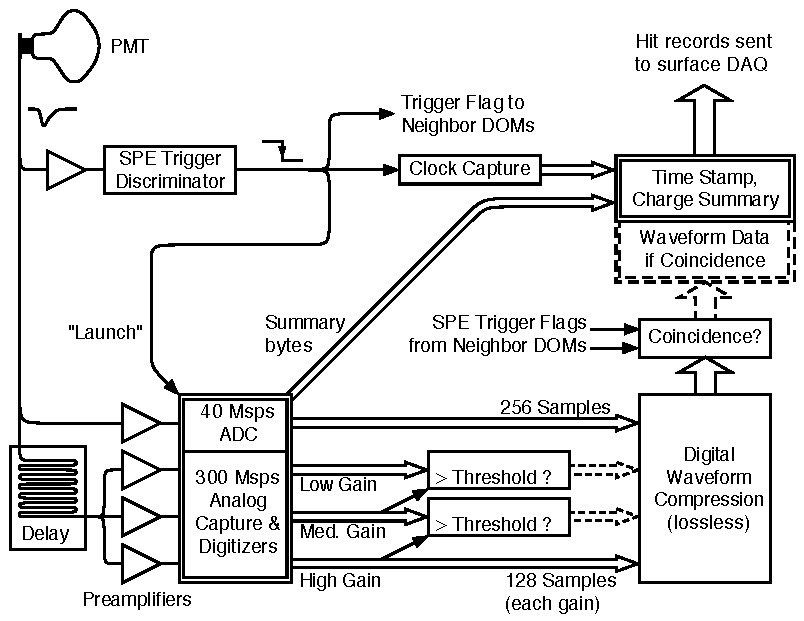
\includegraphics[width=0.9\textwidth]{graphics/dom/functional/domfig3-DOMDataFlow.pdf}
 \caption{Data flow diagram for recording and processing of PMT waveforms in the DOM to form 
 "Hit Records" that are sent to the surface DAQ computers.  As shown by dashes, full waveform data are only included
 when neighbor DOMs report time-coincident signals above the SPE discriminator threshold.  Additionally,
 data from low gain channels are omitted for waveforms that are within range of higher gain channels.}
 \label{fig:domdataflow}
\end{figure}

The ATWD recording duration is \unit[427]ns.  This is sufficient for
reconstructing light produced within tens of meters of
a DOM, but photons from farther away may arrive over a broader time
interval due to the optical scattering of the ice.  Such distant signals are
also lower in amplitude, and the information is captured in the \unit[40]Msps fADC.
The fADC samples continuously, and the FPGA is programmed to save an
interval of \unit[6.4]$\mu$s after the launch. Its amplifier provides a
dynamic range comparable to the high-gain ATWD channel, but has extra pulse shaping to accommodate the lower
sampling speed. An example of a digitized waveform with multiple pulses is shown in
Fig.~\ref{fig:mpe_waveform}.

\begin{figure}[h]
 \centering
 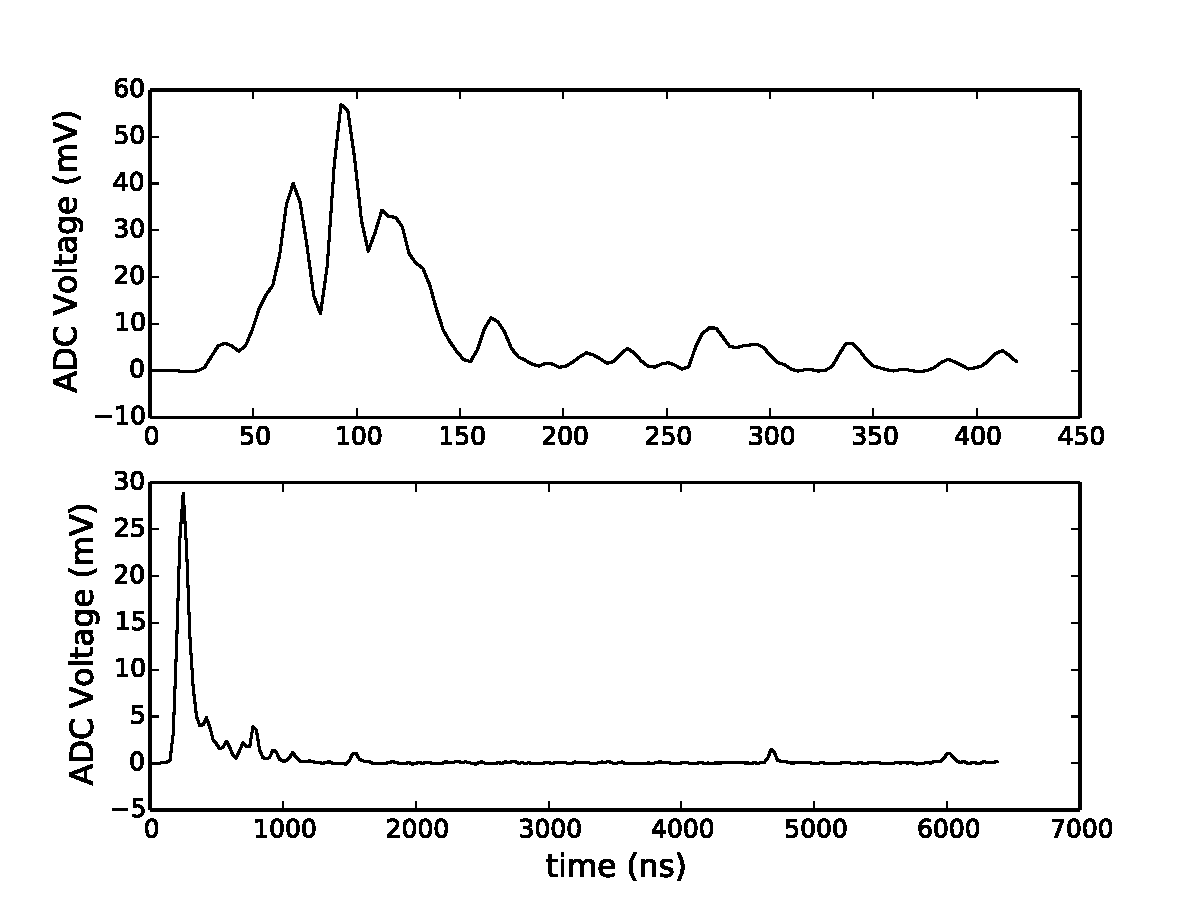
\includegraphics[width=0.9\textwidth]{graphics/dom/functional/mpe_waveform.pdf}
 \caption{Digitized waveforms in the ATWD (top) and the FADC (bottom):
   the ATWD recording duration is 427~ns whereas the FADC recording
   duration is 6.4~$\mu$s. Energy reconstruction in IceCube uses
   the charge and time recorded in the waveform~\cite{IC3:ereco}.}
 \label{fig:mpe_waveform}
\end{figure}

Every digitizer launch results in a ``hit'' record being sent to the surface computers, but the amount of
information included depends on whether a signal was also detected in one of the neighboring DOMs.
In case of an isolated signal (no coincidence), only a time stamp and brief charge summary are sent, and
the digitization process is aborted.  Conversely, when a nearest or next-to-nearest neighbor DOM 
also signals a launch within $\pm$\unit[1]$\mu$s (local coincidence), the full waveform is compressed
and included in the hit record.  The LC signaling operates via digital pulse codes sent on
the extra wire pairs described in Sec.~\ref{sec:penetrator}.

As explained in Ref.~\cite{ICECUBE:DAQ}, two sets of ATWD chips are
operated alternately in order to reduce deadtime; the second ATWD is
available to launch during the digitization step of the first.  Significant deadtime
then only occurs after two back-to-back launches and depends on how many
ATWD channels are digitized, or if the digitization was aborted due to lack
of LC (Fig.~\ref{fig:atwd_timing}).  Therefore, the deadtime depends upon the DOM hit
rate, which varies seasonally based on the atmospheric muon flux~\cite{ICECUBE:IceTop}. 
The median fractional deadtime during a high-rate period for in-ice DOMs
is $6.6\times10^{-5}$, for IceTop low-gain DOMs is $7.2\times 10^{-6}$, and
for IceTop high-gain DOMs is $3.2 \times 10^{-3}$.  

\begin{figure}[]
 \centering
 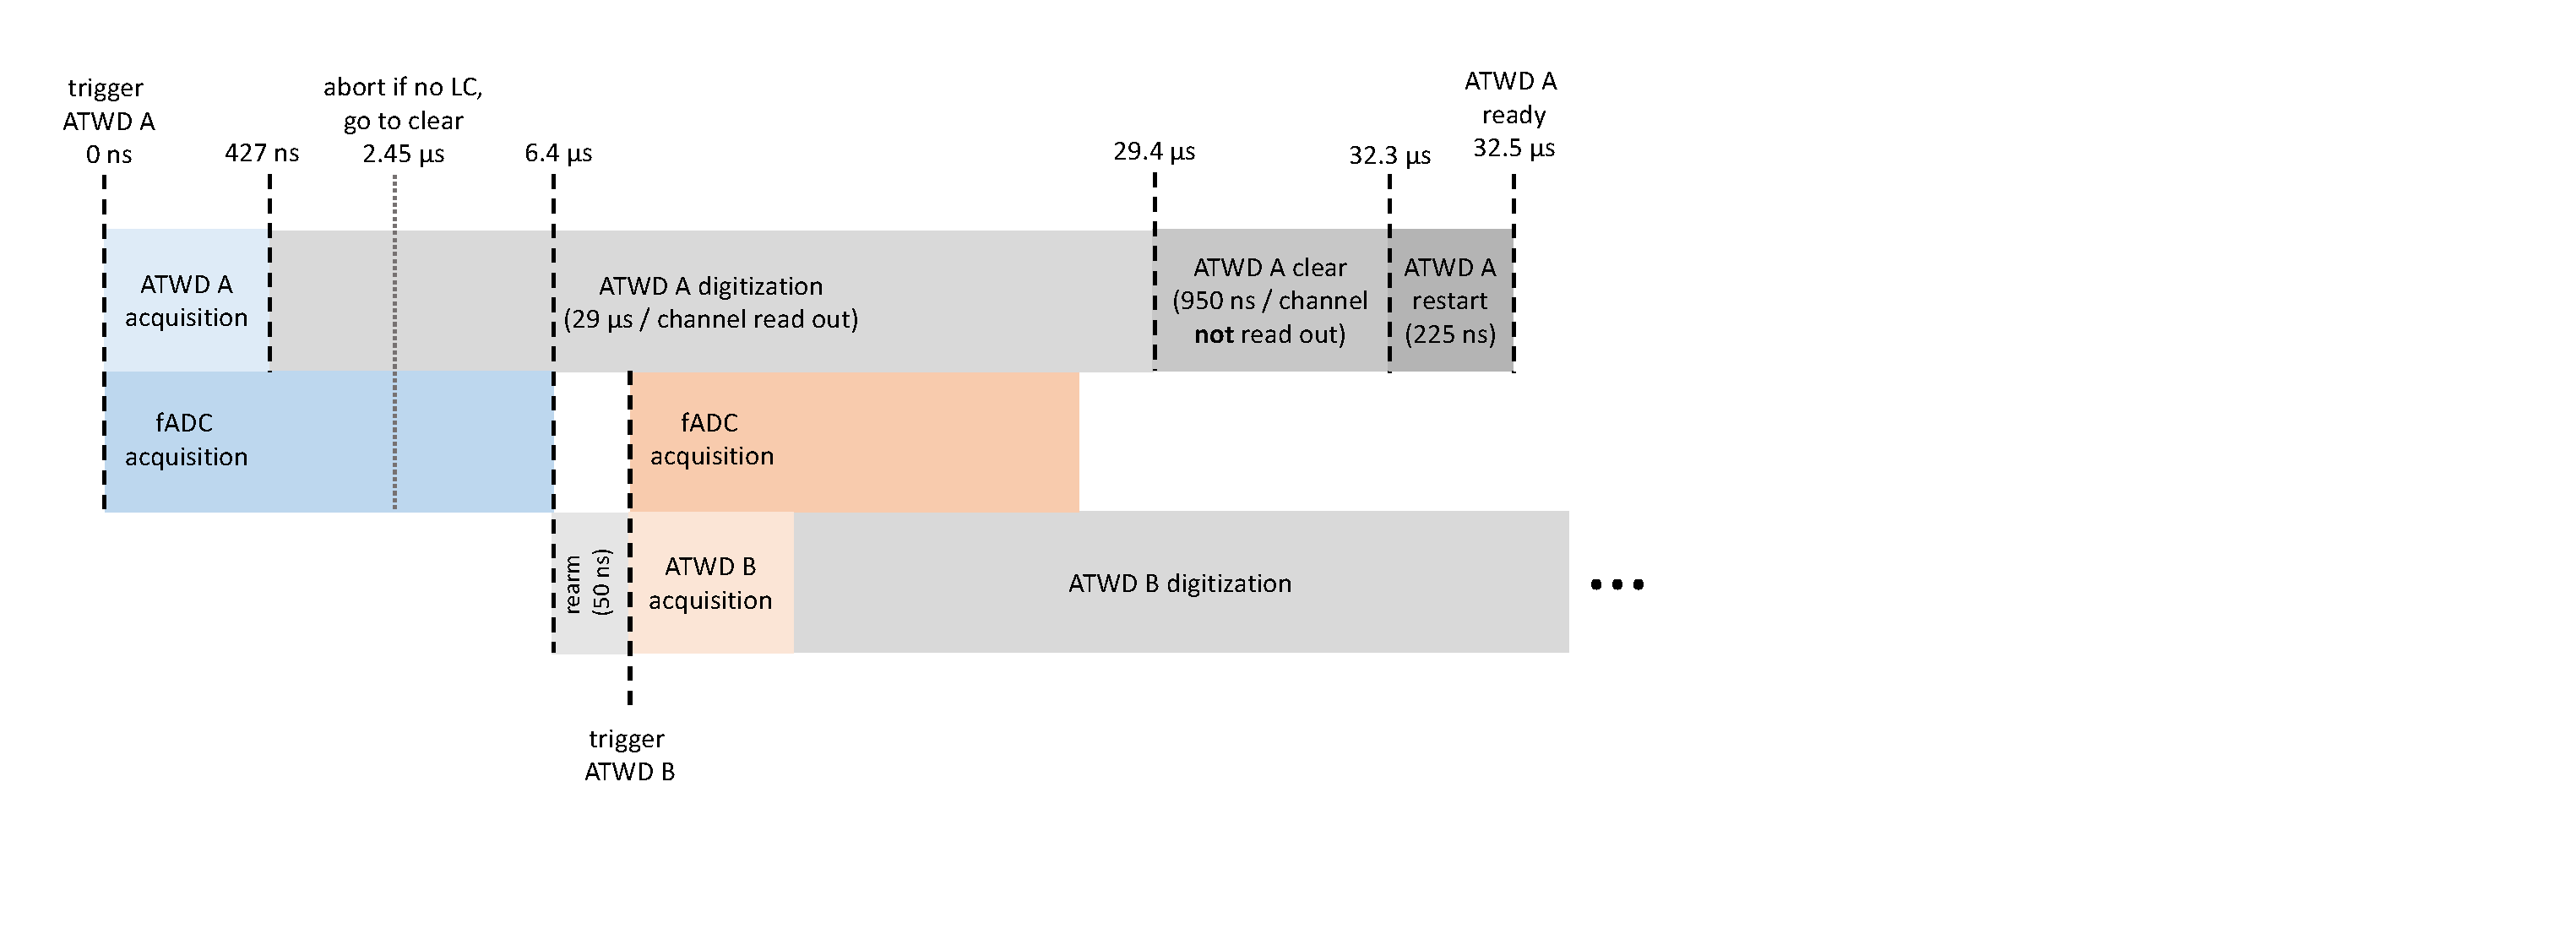
\includegraphics[width=1.0\textwidth]{graphics/dom/functional/atwd_timing.pdf}
 \caption{Timing of ATWD and fADC acquisition and associated deadtime, for
   back-to-back HLC hits with one ATWD gain channel digitized and read out.  The
   horizontal (time) axis is not to scale.}
 \label{fig:atwd_timing}
\end{figure}

\subsubsection{\label{sec:flasher}Flasher Board}

Each DOM contains an LED Flasher Board, which is used to generate
light $in situ$ for a
variety of calibration purposes, including: 

\begin{enumerate}
\item Verifying the timing response of the DOMs throughout the analysis
  software chain.
\item Measuring the position of the deployed DOMs in ice.
\item Measuring the optical properties of the ice.
\item Verifying the performance of shower reconstruction algorithms
  in measuring position, direction, and energy.
\end{enumerate}

The standard Flasher Board, shown in Fig.~\ref{fig:flasherdiagram}, is
included in every DOM except the ``color DOMs''
described below. It is an annular board fitted with 12 LEDs (ETG-5UV405-30)
specified with output wavelength \unit[$405\pm5$]nm.  Laboratory
measurements with sample DOMs yield a peak at
\unit[399]nm and spectral width \unit[14]nm (FWHM) when measured at -20$^{\circ}$~C, where the peak wavelength is shifted by
\unit[$-1$]nm compared to room temperature~\cite{Aartsen:2013rt}.
The LEDs are arranged in pairs, evenly spaced around the board
with a 60$^{\circ}$ separation between each pair. One LED in each pair
is pointed downward at an angle of 10.7$^{\circ}$; after refraction through the DOM glass and into
the ice, the LED
emits light horizontally into the ice. The other LED is tilted upward
at an angle of 51.6$^{\circ}$; after refraction the tilted LED
emits light upward at an angle 
of 48$^{\circ}$, close to the Cherenkov angle in ice. The angular
emission profile of the flasher LEDs was measured in the lab by
rotating a PMT connected to an
optical fiber pickup around the DOM; the readout angle was recorded
using the resistance of a potentiometer at the rotation axis.
The angular emission profile of each LED has a FWHM of
30$^{\circ}$ in air and is modeled as a Gaussian emission profile
with $\sigma = 13^{\circ}$. After refraction through the DOM glass and into
the ice, the emission profile is modified to $\sigma = 9.7^{\circ}$ in the polar direction
and $9.8^{\circ}$ in the azimuthal direction for the tilted LEDs, and $\sigma=9.2^{\circ}$ in the polar direction
and $10.1^{\circ}$ in the azimuthal direction for the horizontal LEDs.
About 10\% of the light is emitted outside the Gaussian beam, modeled by
a secondary profile proportional to $(1+\cos{\alpha})$, where $\alpha$ is the angle
away from the LED axis.

The LEDs are controlled via individual high-speed MOSFET drivers. The LEDs can be turned on individually or in any
combination of the 12, by setting bits in a configuration parameter.
The photon output of each LED depends on the width and
amplitude of the driving current pulse, which are controlled as common
values for all enabled LEDs in each DOM (Figure~\ref{fig:flasheroutput}).  
The pulse width parameter controls the width up to a maximum of \unit[70]{ns}; 
for sufficiently short driving current pulses the light output narrows to \unit[6]{ns} (FWHM) with
10\% afterglow decaying over \unit[15--20]{ns}. The brightness parameter (0--127) controls the driving voltage between
$4.5$ and \unit[15]{V}, which yields a peak current up to
\unit[300]{mA} through the LED and current-limiting resistor.
By varying brightness and width settings as well as the number of LEDs enabled, DOMs can generate flashes
from $10^6$ to $1.4\times10^{11}$ photons, similar to the total light from
neutrino interaction showers between \unit[7]GeV and \unit[1]PeV energy.
The low end of this dynamic range requires fine tuning of driving
parameters in order to operate LEDs very close to threshold.

\begin{figure}[h]
 \centering
 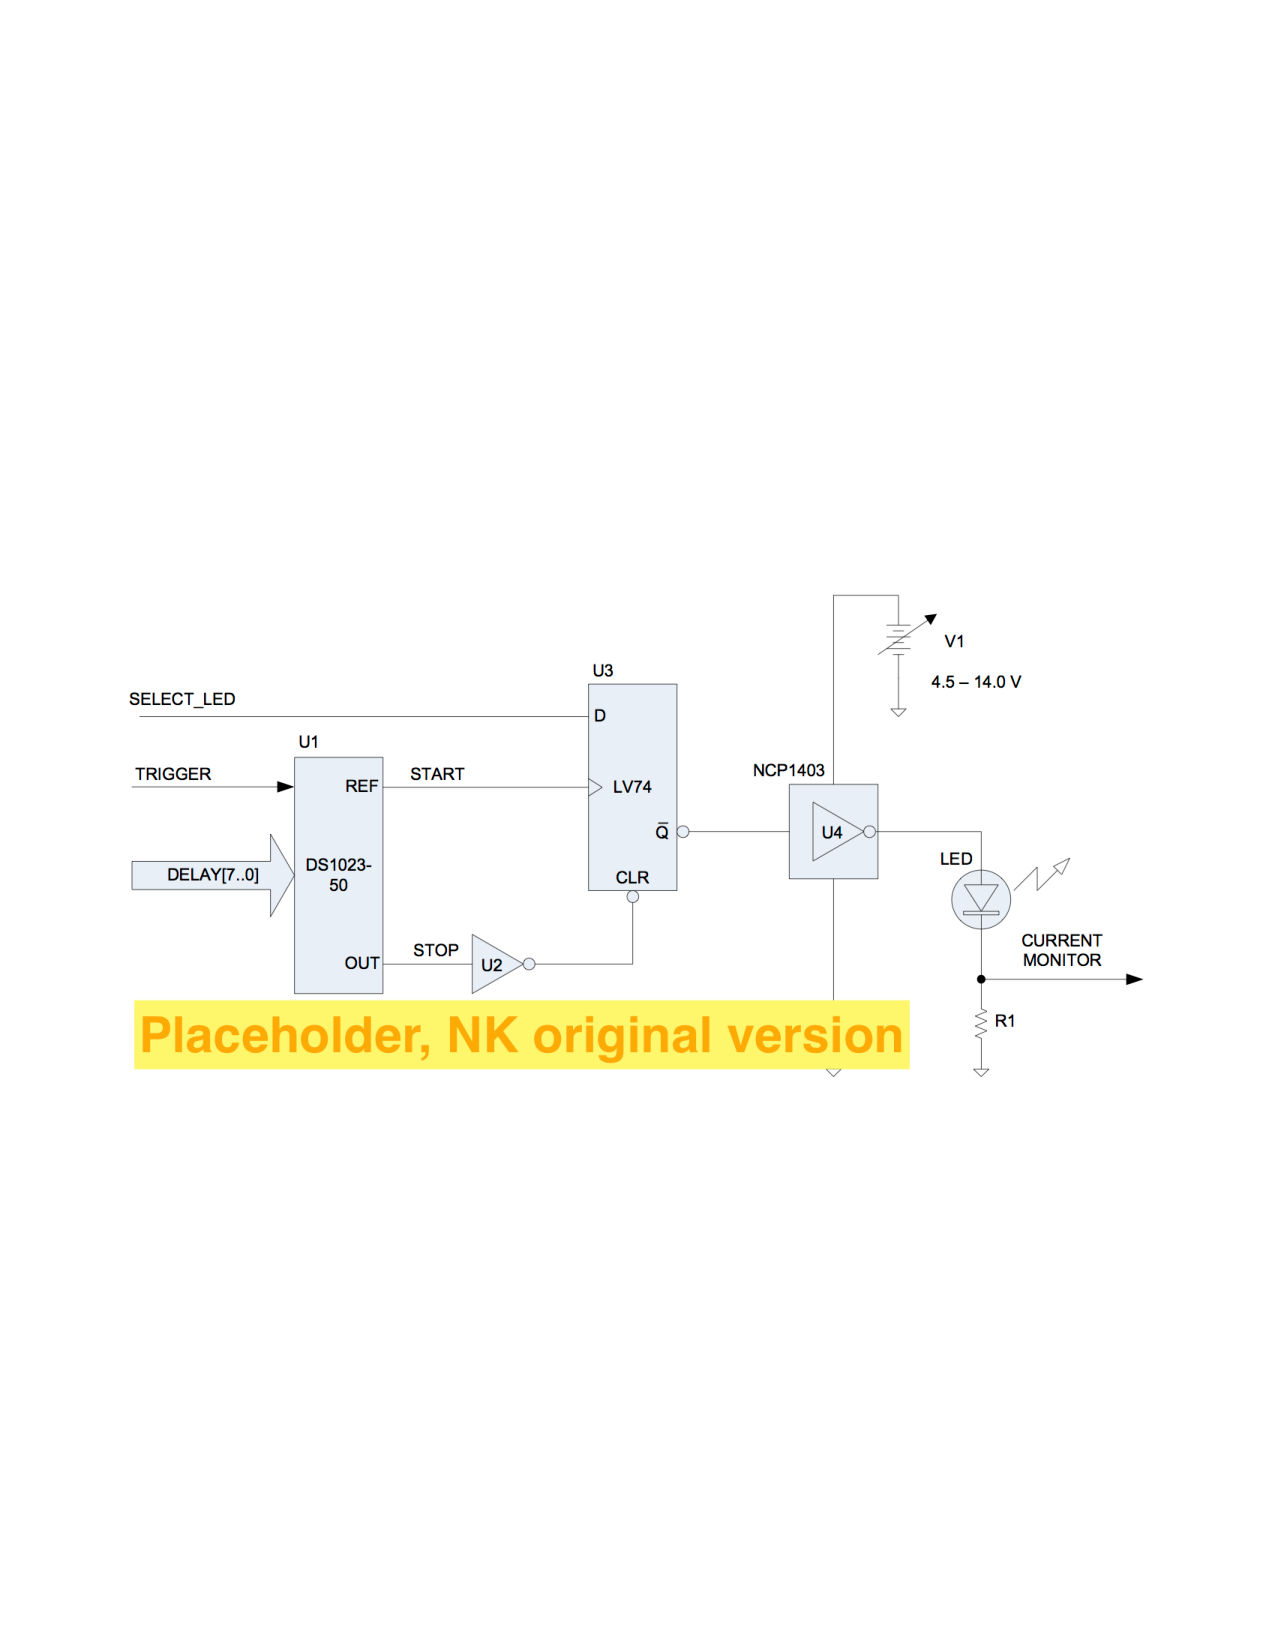
\includegraphics[width=0.8\textwidth]{graphics/dom/functional/domfig4-FlasherDiagram.pdf}
 \caption{LED flasher circuit diagram for one of twelve LEDs, including current pulse monitor (simplified).}
 \label{fig:flasherdiagram}
\end{figure}

\begin{figure}[h]
 \centering
 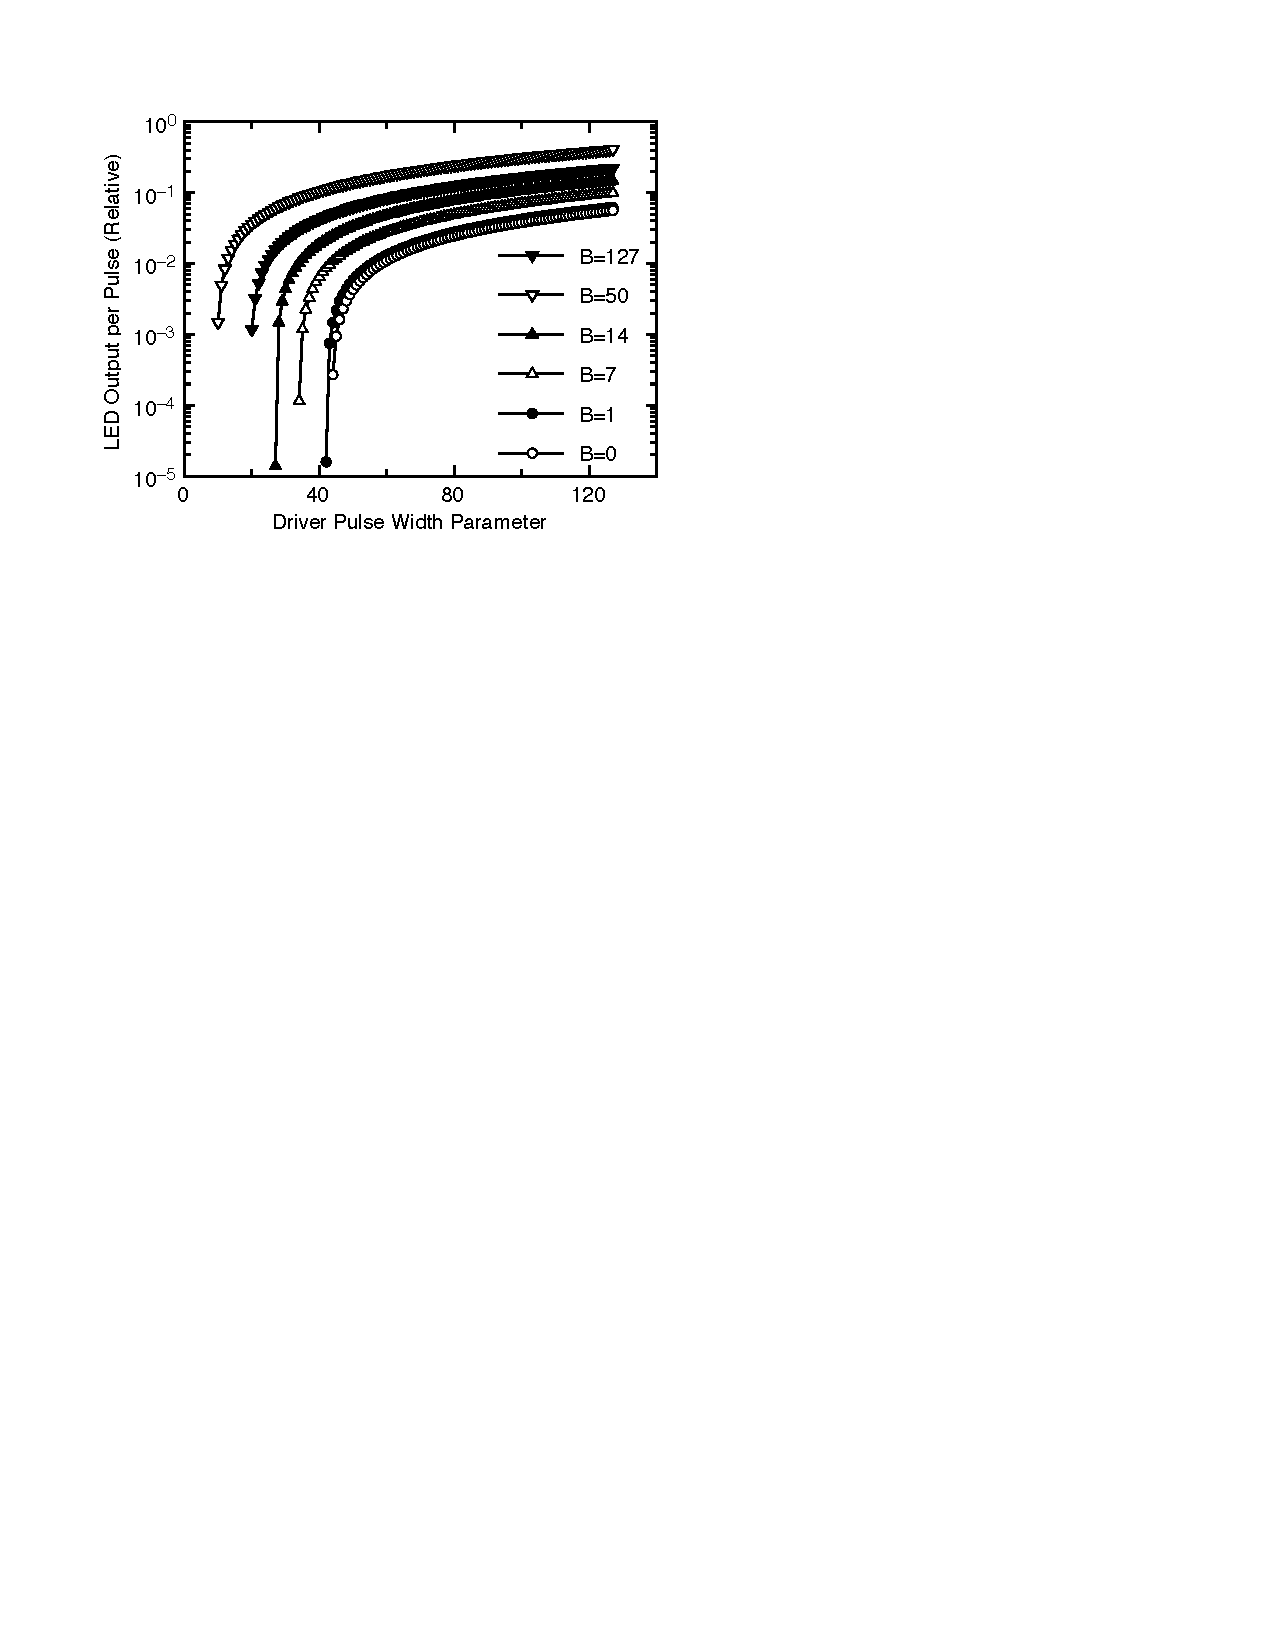
\includegraphics[width=0.6\textwidth]{graphics/dom/functional/domfig5-BrightnessModel.pdf}
 \caption{Light output from flasher LED pulses (relative to maximum), depending
on brightness parameter (B) and width configuration parameters.  Additional dynamic range is available
by enabling from 1 to 12 individual LEDs per DOM.}
 \label{fig:flasheroutput}
\end{figure}

The LED current waveforms are recorded in an auxiliary ATWD channel, supplying
a rising edge time that also establishes the onset of the optical pulse (after a known
turn-on delay).
The repetition rate is programmable up to \unit[610]{Hz}.
Although flashers can be
operated in multiple DOMs in the same run, the DAQ does not support
time-synchronized flashing of LEDs on different DOMs, so coincident flasher
events happen only by chance. 

Sixteen ``color DOMs'' (cDOMs) are fitted with multi-wavelength
Flasher Boards; 8 are deployed on String~79 in the center of IceCube, and 8
are deployed on String~14 on the edge of IceCube.  Each cDOM includes
3 LEDs each with nominal
wavelengths of 505~nm, 450~nm, 370~nm, and 340~nm. The LEDs are arranged in pairs as on the
standard flasher board, but all LEDs point outward horizontally. 
The properties of the LEDs are given in
Table~\ref{table:cdom_properties}.

\begin{table}
\caption{Properties of the standard IceCube flasher LED (tilted (t)
  and horizontal (h)) and the cDOM LEDs, including wavelength $\lambda$,
  emission FWHW $\sigma$ in air, DOM polar
  angular emission FWHM in ice $\sigma_{\theta}$, and DOM azimuthal angular emission
  FWHM in ice $\sigma_{\phi}$.}
\begin{tabularx}{\linewidth}{lXXXXXX}
\toprule
 LED& nominal $\lambda$ (nm) & measured $\lambda$ (nm) & $\sigma$ air ($^{\circ}$) &
 $\sigma_{\theta}$ ($^{\circ}$) & $\sigma_{\phi}$ ($^{\circ}$)\\
\midrule
ETG-5UV405-30 & 405 & 399 & 30.0 & 9.7 (t)& 9.8 (t) \\
 &  &  &  & 9.2 (h)& 10.1 (h)\\
UVTOP335-FW-TO39 & 340 & 338 & 51.0 & 36.1 & 42.9 \\
%\hline
NS370L\_5RFS & 370 & 371 & 55.2 & 39.1 & 42.9 \\
%\hline
LED450-01 & 450 & 447 &	6.8 & 4.8 &	5.3 \\
%\hline
B5-433-B505 & 505 & 494 & 6.4 &	4.5 & 4.9 \\
\bottomrule
\end{tabularx}
\label{table:cdom_properties}
\end{table}

\subsection{\label{sec:dom_prodtest}Production and Testing}

Approximately 5800 DOMs were built and tested, with
approximately 5500 delivered to the South Pole. The DOMs satisfied
stringent requirements, needed to ensure reliable operation in the deep ice
for at least 20 years. As hot-water drilling was the principal 
driver of the deployment timeline, the DOM production schedule was
structured to supply DOMs as needed and to avoid any inventory shortfall.
The production was implemented in a 3-stage approach. Stage 1 was
the production of the initial 400 DOMs at three sites: one in the United
States (Physical Sciences Laboratory (PSL), Stoughton, Wisconsin) and two
in Europe (DESY, Zeuthen, Germany, and Stockholm University,
Sweden). DOM testing was performed at PSL, DESY and Uppsala University,
Sweden. This
quantity of DOMs was sufficient to verify production readiness, supply
instrumentation for the first year drilling plan, and validate the design after a deployment
season.  During Stage 2, material and supplies were procured, and another
1000 DOMs were produced and tested. Finally, Stage 3 involved procurements,
integration, and testing of the remaining DOMs.

DOM production utilized a formalized process to track each DOM through to
the end of the testing process, with each step recorded in a DOM Process
Traveler.  Technicians were trained and certified to perform DOM
integration and test tasks, and each site had separate quality control
personnel. Commercial materials were confirmed to be fully tested by the
suppliers, and regular visits were made to key vendors.  Measurement
equipment was calibrated and records maintained that verified
traceability to a reference standard.  DOM integration took place in
an electrostatic discharge (ESD)-, temperature-, and humidity-controlled environment.  The introduction
of these manufacturing protocols based on electronics industry best
practices enabled each production site to work independently yet
produce DOMs that performed identically.

DOM integration started with the attachment of the PMT collar
to the PMT.  The collar provides a mounting point for the electronic boards inside
a DOM. The PMT was then mounted into a special jig for precise
placement inside the bottom glass hemisphere.  In parallel, the mu-metal
shield was placed inside the bottom hemisphere, and the
gel was mixed and poured into the same hemisphere. The gel was then
degassed by placing under a partial vacuum, in order to avoid bubbles and
cracks (``crazing'') in the gel. 
After degassing, the PMT was placed in the gel and allowed to cure for 48
hours.  After curing, the PMT Base Board was soldered onto the leads of the
PMT.  Separately, the PC Board Stack was assembled by attaching the Delay
Board, Main Board, Flasher Board, and High Voltage Control Board together.
The Board Stack was then mounted onto the PMT collar, the penetrator assembly
was mounted into the top hemisphere, and the two halves of the sphere were
joined.  With the entire assembly under a bell jar, the spheres were
evacuated and backfilled with dry nitrogen, 
a butyl rubber sealant applied around the seam, and the seam covered with
wide plastic tape. The interior gas pressure was reduced to 0.5 bar (at
room temperature) so that the seal remains tight even at the assumed minimum
ambient South Pole air pressure of 0.64 bar.

As the DOMs are not serviceable after deployment, an extensive testing
protocol (Final Acceptance Testing, or FAT) including temperature-cycling
and cold-soaking ensured that bad modules and early component failures were
identified and repaired before shipping.  This testing at production sites
was performed in Dark Freezer Labs (DFLs), light-tight walk-in 
modules capable of sustaining temperatures down to $-55^\circ$C.  Main Board
and DOM functionality was tested by self-diagnostic software installed on
each module.  Other tests included gain calibration, dark noise monitoring,
and LC validation.  Optical sensitivity, time resolution,
and linearity were measured using external light sources fed into the DFLs
via optical fibers and diffused over the DOM lower hemispheres at each
testing station. Sensitivity was measured primarily with a
monochromator-selected white lamp; time resolution was measured with a
pulsed diode laser (405~nm), and linearity was measured with a bright
pulsed LED source (405~nm).

A typical FAT temperature and testing cycle is shown in
Fig.~\ref{fig:fat_cycle}. The initial pass rate of DOMs during FAT was
92\%.  The primary causes of failures were elevated noise rates detected during the
low-temperature soak, functional issues on the Main Board or Flasher Board,
and PMT gain instability.  The majority of failing DOMs were retested and
subsequently passed, while DOMs with serious issues were repaired and
retested prior to shipment. After the successful completion of FAT, DOM
deployment harnesses were attached (see Fig.~\ref{fig:domcable}) and the DOMs individually packed. 

\begin{figure}[!h]
 \centering
 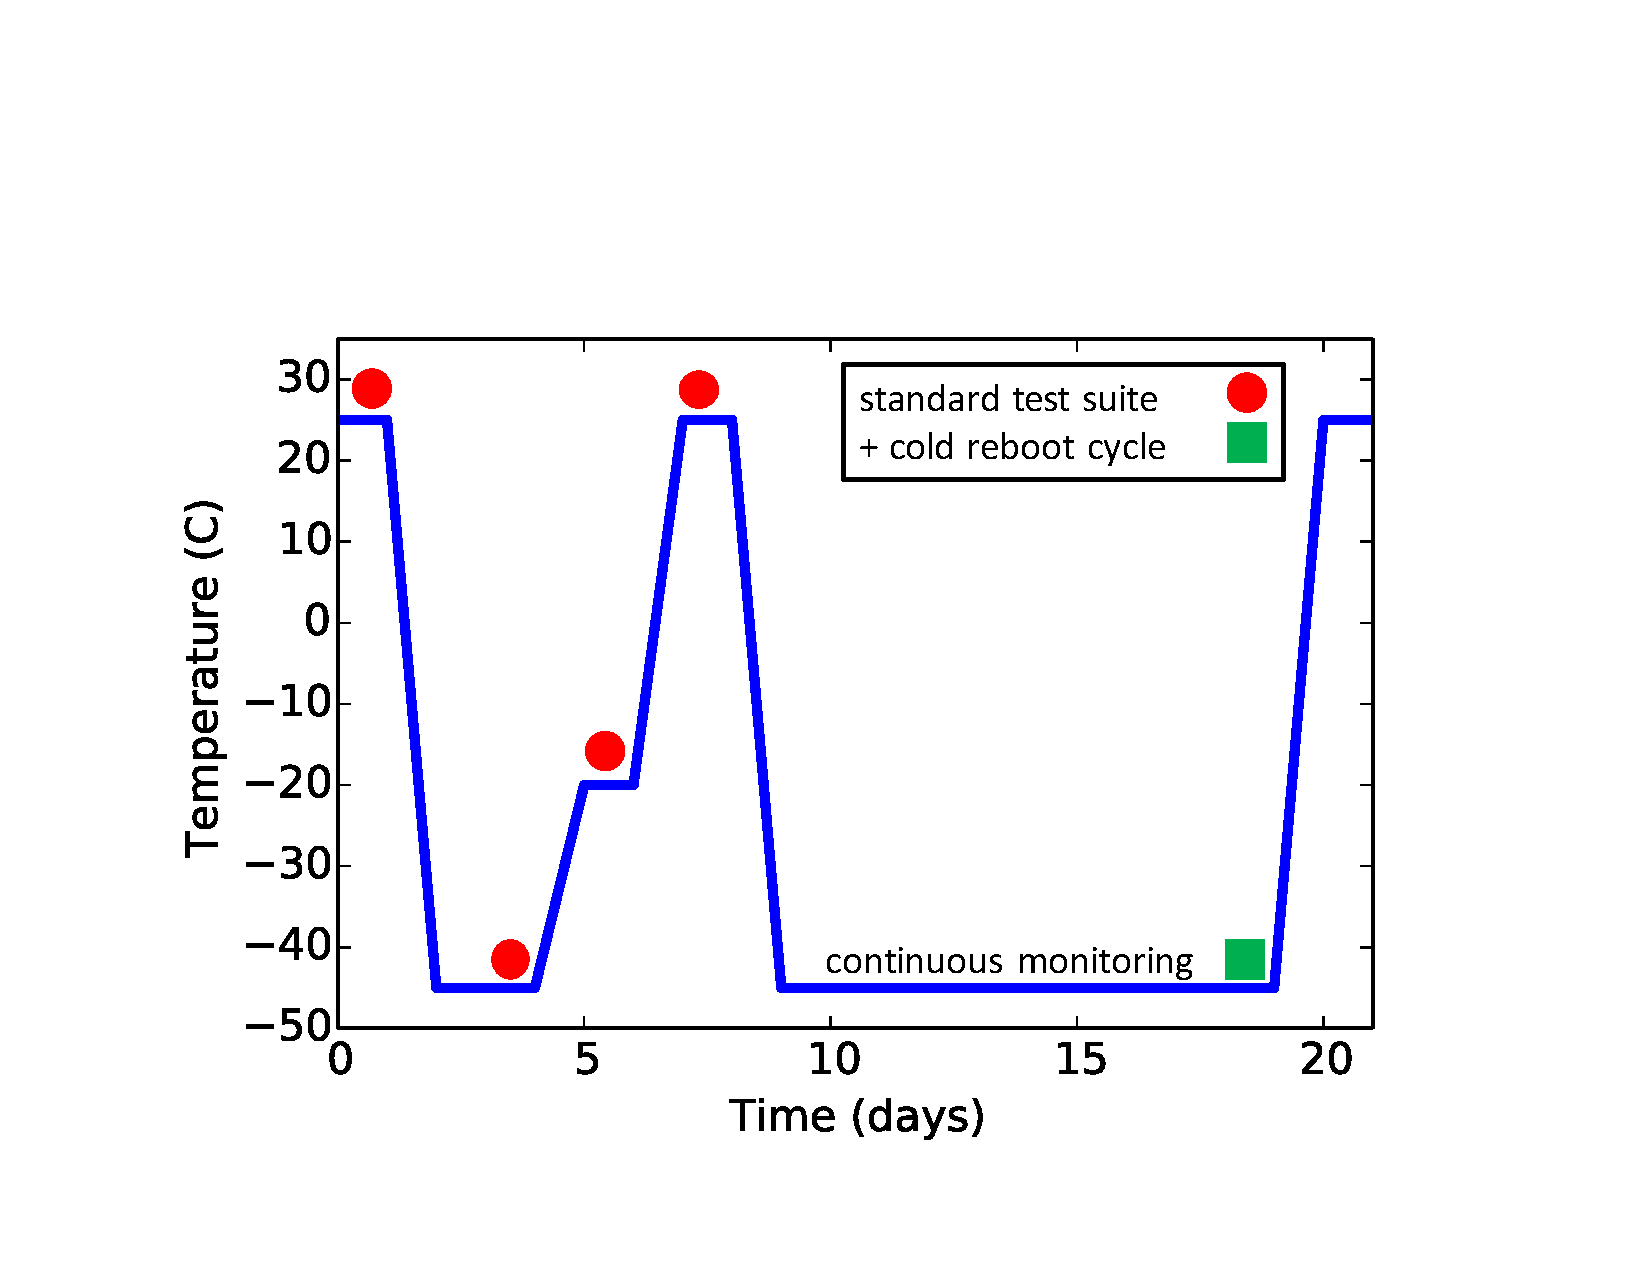
\includegraphics[width=0.6\textwidth]{graphics/dom/production/fat_cycle.pdf}
 \caption{Final Acceptance Testing (FAT) temperature profile, including
   testing steps performed at each stage.}
 \label{fig:fat_cycle}
\end{figure}

All DOMs were also re-tested at the South Pole before final deployment, to
screen out any modules damaged during transit.  The self-diagnostic
program and dark noise measurements were performed with the DOMs still in
their packing boxes, covered with additional light-tight material.  Of the
approximately 5500 DOMs shipped to South Pole, about 30 (0.5\%) were
returned to the U.S.~after failing on-ice testing.    

\subsection{\label{sec:reliability}Reliability}

As of 2016, 5397 of the 5484 deployed DOMs ($98.4\%$) are operating in
data-taking mode in the data acquisition system; the remaining 87~DOMs
have failed (see Table
\ref{tab:dom_failures}).  We classify DOM 
failures into two broad categories: failures during deployment and
freeze-in, and failures during subsequent operation.  The majority of the
failures (55) occurred before post-deployment commissioning; we hypothesize
that these are primarily attributable to cable failures, water leaks,
or freeze-in damage. 32 DOMs have failed after commissioning, and
we include in this count modules on a wire pair taken out of service when
the partner DOM on the same pair failed.  No particular pattern in the
failures is observed, other than they are typically during non-standard
operation or an exceptional event: a power outage, calibration run, or
flash filesystem upgrade.  The most recent two DOMs failed on May 23, 2013,
losing communications after a power outage.  Diagnosis of DOM failures
beyond identifying electrical shorts is challenging.

A total of 171~DOMs have developed issues that affect their data-taking
configuration but are still usable.  For example, DOMs with a single functional
ATWD chip have a higher deadtime but are otherwise good.  The LC settings of functional DOMs adjacent on a string to
dead DOMs must also be modified. In most cases, local coincidence is
disabled in the direction of a dead neighbor DOM, but in a few cases a
malfunctioned DOM can still be configured to forward the local
coincidence signals along the string even if it is not used in
data-taking. These are enumerated in Table \ref{tab:dom_failures}.  

\begin{table}[h]
  \centering
  \caption{Number of DOM failures during deployment/freeze-in and after
    commissioning during detector operation, as well as DOMs with various
    issues (including a failed neighbor) causing them to be operated in a
    non-standard data-taking mode.} 
  \label{tab:dom_failures}
  \begin{tabular}{rc|rc}
    \toprule
    DOM failures & N & DOMs in non-standard mode & N\\
    \hline    
    deployment / freeze-in & 55 &single functional ATWD & 12\\
    post-commissioning & 32  & reduced PMT gain & 1 \\
   & & non-standard LC & 158 \\
 total & 87 & total& 171\\
    \bottomrule 
  \end{tabular}
\end{table}

We can estimate the surviving fraction of DOMs 25 years after the original
deployment, assuming a constant, random failure rate after freeze-in.
Specifically, we calculate the Wilson score binomial confidence interval \cite{Wilson_Score} of
survival probability using the post-commissioning failure rate of DOMs.
The estimated survival fraction as a function of 
time is shown in Fig.~\ref{fig:dom_survival}.  Currently we estimate the
mean failure rate to be $4.1\pm1.2~\mathrm{yr}^{-1}$, resulting in a
survival fraction in 2030 of $97.4\pm0.3\%$.  While this simplified 
model does not account for an increase in failure rate due to component aging, the
recent observed failure rate since detector completion of $1.7~\mathrm{yr}^{-1}$ is
significantly lower than the mean predicted rate, since the failure rate
during construction was higher.  We attribute
this to infant mortality and/or to improved operational protocols that
minimize the number of DOM power cycles.  DOMs are not regularly
power-cycled during data-taking but only when required to resolve an
intermittent problem.

\begin{figure}[!h]
 \centering
 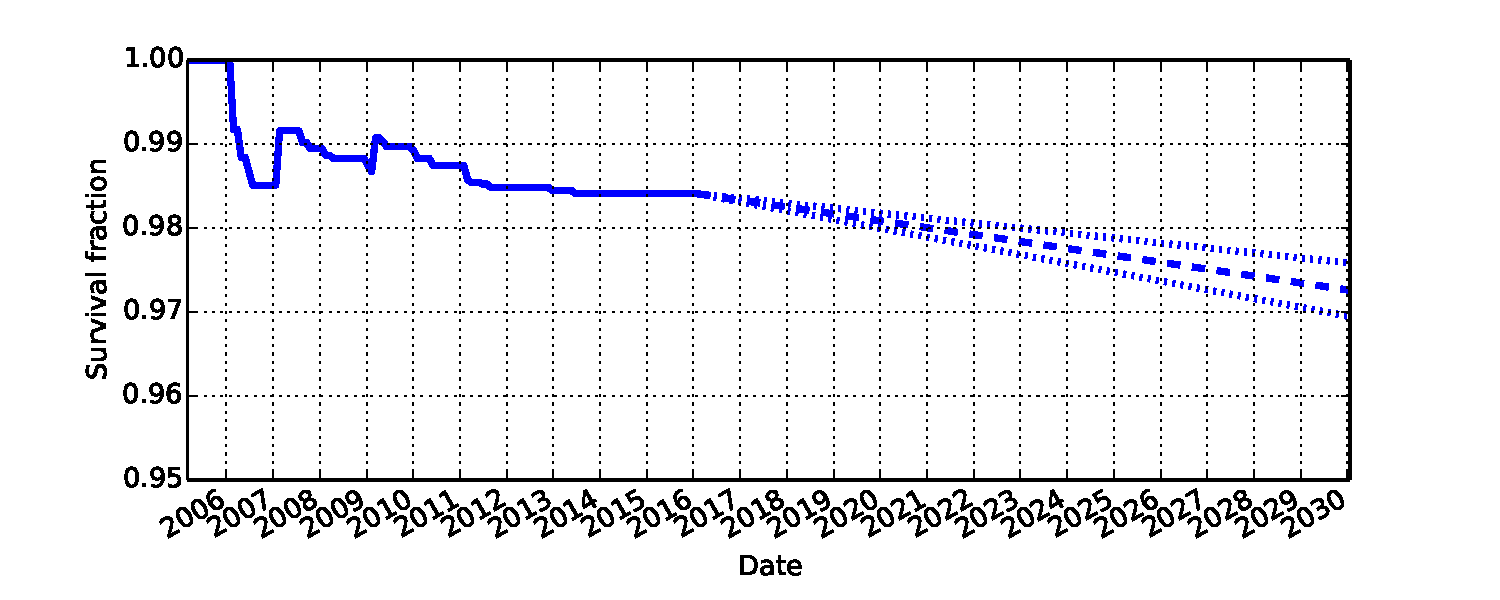
\includegraphics[width=0.95\textwidth]{graphics/dom/reliability/dom_survival.pdf}
 \caption{Actual and predicted fraction of surviving DOMs versus time, based on an assumed
 constant post-freeze-in failure rate.  The dotted lines indicate the
 central and 95\% CL estimates.  Increases before 2011 are due
 to deployments of new strings.} 
 \label{fig:dom_survival}
\end{figure}
